\documentclass[10pt,a4paper]{article}
\usepackage[T1]{fontenc}
\usepackage{lmodern}
\usepackage[a4paper,left=18mm,right=18mm,top=18mm,bottom=18mm,headheight=13pt,headsep=6mm]{geometry}
\usepackage{graphicx,booktabs,tabularx,array,amsmath,amssymb,enumitem,xcolor,caption,fancyhdr,microtype}
\usepackage[hidelinks]{hyperref}
\usepackage{xurl}
\definecolor{teal}{HTML}{087E8B}
\definecolor{ink}{HTML}{163746}
\definecolor{light}{HTML}{EDF5F6}
\pagestyle{fancy}\fancyhf{}
\fancyhead[L]{\small\color{ink}EE5110 Segment C\enspace |\enspace Autonomous Robot Manipulation}
\fancyhead[R]{\small Final report}
\fancyfoot[L]{\scriptsize Simulation, physical execution and paired evidence}
\fancyfoot[R]{\small\thepage\,/\,10}
\renewcommand{\headrulewidth}{0.4pt}
\setlength{\parindent}{0pt}\setlength{\parskip}{5pt}
\setlist[itemize]{leftmargin=14pt,itemsep=2pt,topsep=3pt}
\setlist[enumerate]{leftmargin=16pt,itemsep=2pt,topsep=3pt}
\captionsetup{font=small,labelfont=bf,skip=4pt}
\renewcommand{\arraystretch}{1.17}
\newcolumntype{Y}{>{\raggedright\arraybackslash}X}
\newcommand{\pageheading}[2]{{\Large\bfseries\color{ink}#1\quad #2}\par\vspace{3pt}}
\newcommand{\takeaway}[1]{\par\vspace{3pt}\noindent\colorbox{light}{\parbox{\dimexpr\linewidth-2\fboxsep\relax}{\small\textbf{Finding.} #1}}\par}
\newcommand{\code}[1]{\nolinkurl{#1}}
\newcommand{\subhead}[1]{\par\vspace{3pt}{\bfseries\color{teal}#1}\par}
% Optional real group name and member identities may be added here by the team.
\newcommand{\TeamLine}{EE5110 Segment C --- Group Project}
\begin{document}
\thispagestyle{fancy}
{\huge\bfseries\color{ink}Autonomous Manipulation\\[3pt]Beyond a Successful Grasp\par}
\vspace{5pt}
{\large Geometric alternatives, robust observations and contact-aware execution\par}
\TeamLine\hfill 27 October 2026

\subhead{Abstract}
A simulated grasp is useful only if the robot can hold, transport and release the object under declared physical constraints. We implement a complete MuJoCo--Franka Panda pipeline using public YCB objects, numerical inverse kinematics, collision-checked motion and contact-driven execution. We then investigate three failure bottlenecks: blocked grasp approaches, corrupted range observations and inadequate contact retention. In a frozen 180-episode paired study, bounded inclined/offset candidates complete 58/60 three-neighbor tasks and 29/30 five-neighbor tasks, versus 54/60 and 26/30 for the original candidates. A separate 126-episode exploratory study finds that indiscriminate depth fusion can degrade success to 1/12, whereas cross-packet voxel support reaches 9/12; contact regulation completes 6/6 elastic-object tasks versus 2/6 with fixed preload. Controlled closure-fault recovery, passive articulated objects and procedural unknown shapes provide additional mechanism evidence. Negative results and wide confidence intervals qualify these observations: no paired comparison passes its stated multiple-comparison threshold, and simulator geometry remains available to planning. The result is a reproducible investigation of where the pipeline fails and which bounded interventions help, rather than a universal grasping claim.

\begin{center}
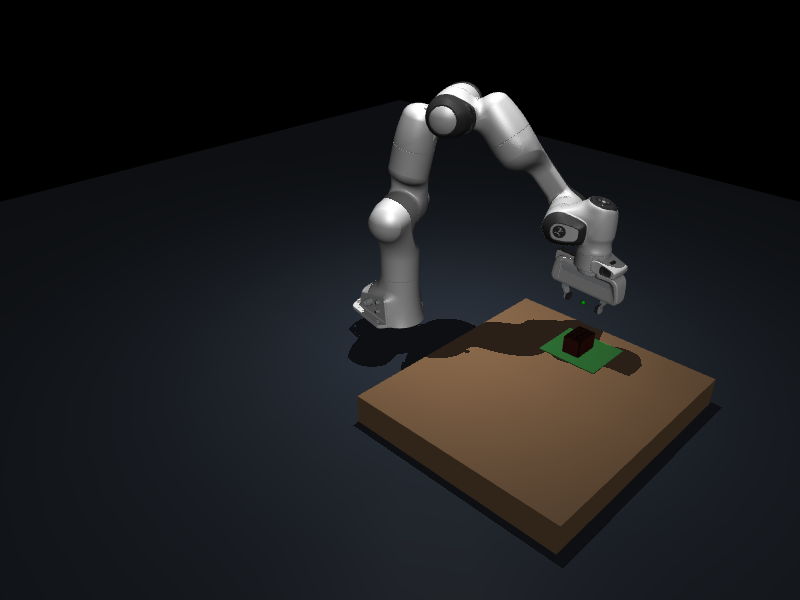
\includegraphics[width=.72\linewidth,height=60mm,keepaspectratio]{figures/workcell.png}
\captionof{figure}{Contact-based Panda pick-and-place workcell with a public YCB object. This is an illustrative development snapshot, not an additional evaluation trial.}
\end{center}

\subhead{Research questions and report structure}
\begin{tabularx}{\linewidth}{@{}p{16mm}Yp{28mm}@{}}
\toprule Question & Investigation & Evidence \\
\midrule RQ1 & Can a small local grasp family avoid palm--neighbor collisions without changing the planner or physical gates? & 180 episodes; p.~4 \\
RQ2 & When depth errors are correlated, does geometrical consistency matter more than the number of observations? & 3 sensing arms; p.~6 \\
RQ3 & Can bounded contact regulation and checked retries retain objects and recover a transient execution fault? & Soft/force/retry; pp.~5,7 \\
\bottomrule
\end{tabularx}
\takeaway{Task-level evidence must connect perception, motion and contact. More candidate poses, more observations or a high intermediate confidence score are not independently sufficient.}

\newpage
\pageheading{1}{System, assets and task definition}
\subhead{Baseline workcell and public object dataset}
The workcell uses MuJoCo contact dynamics, a seven-joint Franka Panda and actuated parallel fingers, a support table, and a destination region. The Panda asset is pinned to Menagerie commit \code{0059d4335f8156206f63a35662313385f7ad6d74}; dataset conversion assets are pinned separately and retain their upstream licenses \cite{mujoco,menagerie,ycb,conversion}. The public YCB subset contains foam brick, gelatin box, pudding box, tomato soup can, lemon and strawberry. The baseline entry point supports seeded random object selection, translation and yaw; primitive cubes are only development checks. In the clutter studies, three box-like objects are balanced manipulation targets and the remaining models form three or five simultaneously active distractors. The YCB foam-brick mesh is a rigid object; the genuinely elastic model on page 5 is a separate model.

Targets spawn at $x\in[0.43,0.52]$ m and $y\in[-0.105,-0.065]$ m in the clutter protocol, with randomized yaw and bounded neighbor-layout jitter. The destination center is $(0.48,0.30)$ m. A barrier and two posts constrain transfer. Distractors retain free-body dynamics, gravity and collision. These are structured tabletop layouts, not arbitrary stacked piles.

\subhead{Coordinate convention and modular pipeline}
We use $T^A_B\in SE(3)$ to map coordinates from frame $B$ to frame $A$: $\bar p^A=T^A_B\bar p^B$. An estimated object transform $\widehat T^W_O$ and object-frame geometry produce world-frame candidate grasp transforms. During scratch-state planning, the relative object--gripper transform predicts a held object; this hypothetical geometry update never attaches or teleports the live object.
\begin{center}
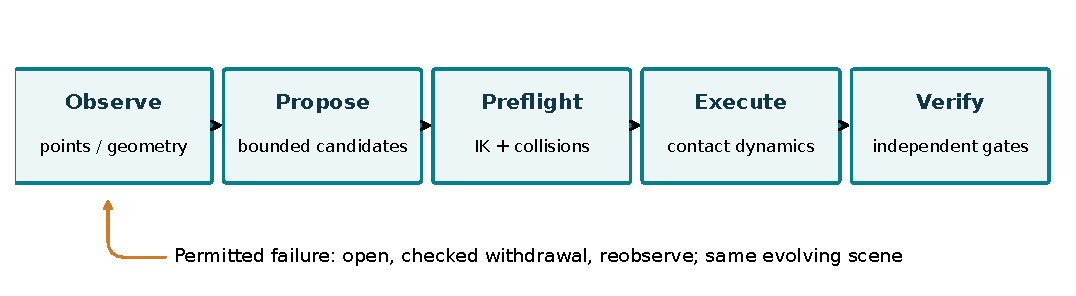
\includegraphics[width=\linewidth]{figures/pipeline.pdf}
\captionof{figure}{Module responsibilities and permitted recovery. Outcome verification is separate from grasp selection and controller commands.}
\end{center}

\begin{tabularx}{\linewidth}{@{}p{30mm}Yp{45mm}@{}}
\toprule Stage & Information and decision & Main implementation \\
\midrule Scene/data & Load pinned assets; seed object identity, pose and materials; settle once. & \code{environment.py}, \code{dataset.py} \\
Observation & Estimate pose/extent from declared point inputs, or isolate mechanics with simulator geometry. & \code{active_sensing.py}; \code{exploration/sensing.py} \\
Grasp/planning & Generate candidates; solve IK; reject unsafe approach and downstream motion. & \code{grasp.py}, \code{local_grasps.py}, \code{planning.py} \\
Execution & Approach, close, lift/hold, transfer, lower, open and retreat using actuators. & \code{control.py}; \code{exploration/manipulation.py} \\
Evaluation & Retain failures, physical gates, contact/force traces, seeds and source fingerprints. & \code{evaluation.py}; evidence audit scripts \\
\bottomrule
\end{tabularx}

\subhead{What counts as baseline completion}
The course baseline requires a simulated workcell, randomly selected public-dataset objects, generated grasp poses, robot execution and repeated randomized evaluation \cite{brief}. All five are implemented. Additional studies change a declared bottleneck while preserving outcome checks. A planner rejecting a collision before motion is a recorded failure to complete the task, even though the safety behavior is correct.

\newpage
\pageheading{2}{Observation, planning and physical verification}
\subhead{Declared sensing interfaces}
The simplest dataset baseline uses known geometry and pose. The clutter estimator instead receives measured range points and a known upright box template. Calibrated $96\!\times\!96$ orthographic rays, ideal simulator instance masks and a synthetic corruption model generate the points: 98\% independent missing returns, 10\% persistent missing pixels per view and 0.5 mm height noise. Active acquisition processes eight-frame batches, with 16--64 frames and up to three fixed virtual views. Acceptance requires at least 48 distinct footprint points, footprint error $\leq6$ mm, consecutive position change $\leq3$ mm and yaw change $\leq0.08$ rad. No missing-data fallback inserts the true pose into this estimator.

The procedural point-only observer on page 6 has no target CAD or instance labels. Nevertheless, all planners access simulator collision geometry, and transfer centering accesses the simulated target center. Material, force, recovery and hinge studies use simulator geometry to isolate mechanics. Thus the system is \emph{point-based grasp estimation with simulation-assisted planning}, with the observation interface varied explicitly by experiment. Ray capture does not advance physical time; frames divided by a nominal frame rate are not measured camera latency.

\subhead{Grasp generation and bounded motion planning}
Mesh projections determine aperture plus a 6 mm margin, limited to 80 mm. Original top candidates use yaw offsets $0,\pi/2,\pi/4,-\pi/4$; pregrasp clearance is 140 mm and nominal lift distance is 160 mm. Candidate previews check the pregrasp, approach and downstream task before execution. Numerical IK uses damped least squares,
\begin{equation}
\Delta q = J_w^\top(J_wJ_w^\top+\lambda^2 I)^{-1}e_w,\qquad \lambda=0.025,
\end{equation}
with orientation weighted by 0.4. Up to nine seeds, 500 iterations, 2 mm position and 0.025 rad rotation tolerances bound the search. Static collision rejection accompanies IK. Joint-space edges are sampled at about 0.015 rad maximum joint increment. Bounded bidirectional RRT-Connect is available for constrained transit; these discrete checks are not a continuous collision-safety proof.

Actuator references follow $q(\alpha)=q_0+(3\alpha^2-2\alpha^3)(q_1-q_0)$. Timing bounds the \emph{commanded} joint trajectory at 0.5 rad/s and 2 rad/s$^2$; actual dynamics are independently checked. Live manipulation uses contact forces without robot--object weld, adhesion or teleportation.

\subhead{Independent complete-task gates}
\begin{tabularx}{\linewidth}{@{}p{32mm}Y@{}}
\toprule Requirement & Recorded criterion \\
\midrule Lift and hold & Height $>80$ mm above the original reference throughout a 1 s hold; bilateral contact on $\geq95\%$ of hold samples. \\
Release and placement & Fingers disengaged; object supported by table; XY destination error $<55$ mm; speed $<20$ mm/s after settling. \\
Actuation & Peak gripper actuator force $\leq40$ N; this is not a per-finger normal-force bound. \\
Clutter preservation & Maximum neighbor translation $\leq20$ mm, zero unsafe-contact steps and target/environment penetration $\leq1$ mm. \\
Elastic extension & Peak absolute edge strain $\leq40\%$ in addition to all applicable grasp/place checks. \\
\bottomrule
\end{tabularx}
\takeaway{A detected grasp, reached pose or successful lift alone does not satisfy complete pick-and-place success. The same declared gates are applied to both arms of each paired comparison.}

\newpage
\pageheading{3}{RQ1: bounded geometric alternatives in clutter}
\subhead{Diagnosis before intervention}
In a reproducible development failure, both original candidates were rejected during approach: each of nine IK seeds produced palm contact with the nearby tomato-soup can. The diagnostic collision penetration was approximately 0.5--1.3 mm; no live motion was executed. The apparent IK failure therefore exposed a blocked candidate family, rather than proving that all grasps were unreachable. This distinction motivates changing the candidate geometry while preserving the planner and execution checks.

\subhead{Local candidate construction}
The original candidates retain their order and priority. For vertical approaches, the generator appends at most 16 alternatives by rotating about the closing axis through $\pm30^\circ$ or $\pm45^\circ$, and shifting the pad center by $\pm12$ mm along the other horizontal axis. It requires at least 10 mm remaining template support and checks projected width plus the original 6 mm margin against the 80 mm aperture. The generator uses the estimated pose and template mesh, without reading target true pose or neighbor geometry. Full collision and downstream previews still reject each unsuitable proposal. Candidate expansion is a finite local search, not general six-dimensional grasp synthesis or rearrangement.

\begin{center}
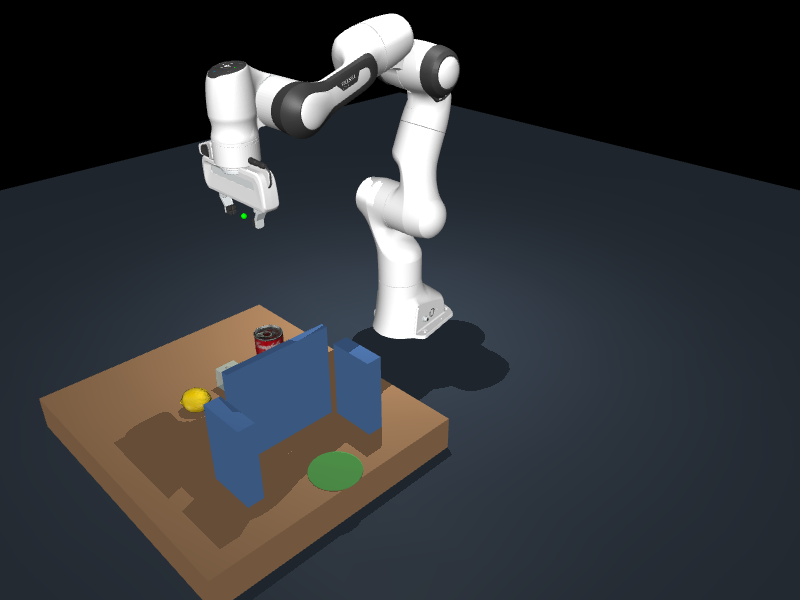
\includegraphics[width=.43\linewidth,height=40mm,keepaspectratio]{figures/rejected.png}\hfill
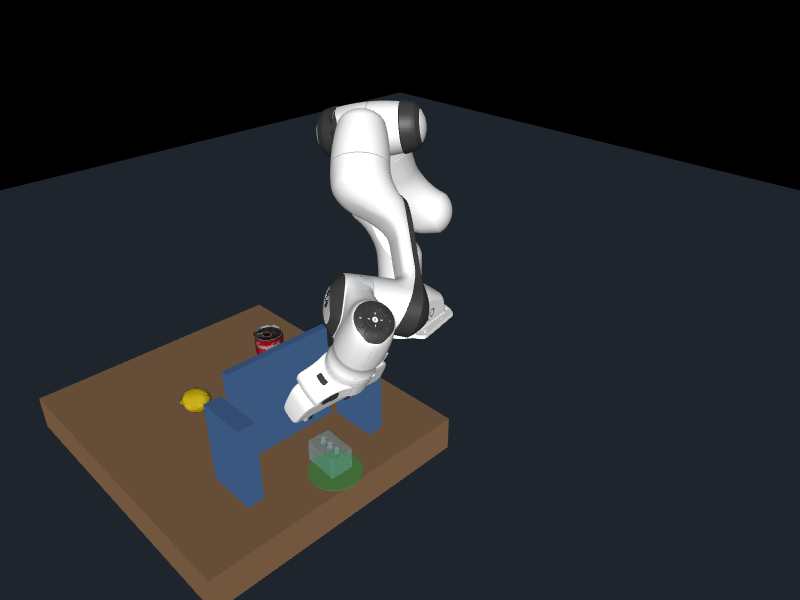
\includegraphics[width=.43\linewidth,height=40mm,keepaspectratio]{figures/inclined.png}
\captionof{figure}{Same development scene: original candidates are safely rejected (left); an inclined alternative completes physical release (right). Root seed 20261608; both examples are excluded from the formal study below.}
\end{center}

\subhead{Frozen paired study: 180 physical episodes}
Root seed 20261025 yields 60 three-neighbor scenes per method and 30 five-neighbor scenes per method, balanced over the three target models. Exact settled scenes, estimates and scene/sensor/planner seeds are paired. Both arms use active observations, ordinary control and one attempt; \emph{only candidate strategy changes}. All failures remain in the denominator.
\begin{center}
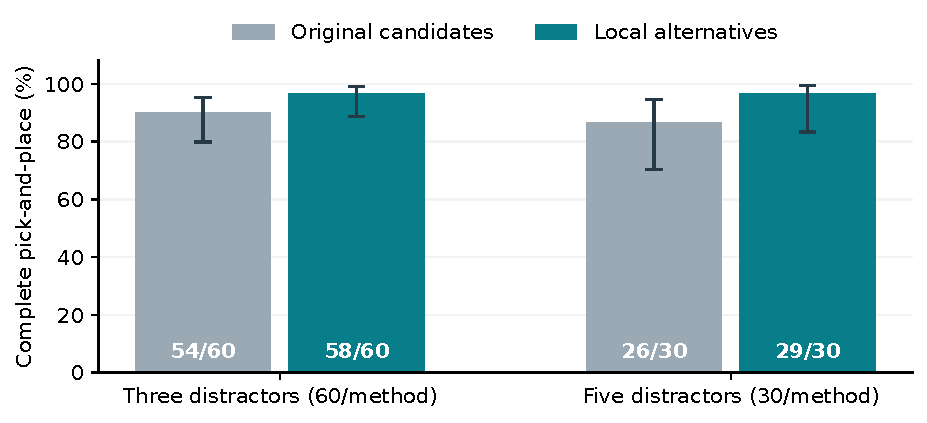
\includegraphics[width=.82\linewidth,height=49mm,keepaspectratio]{figures/candidate_results.pdf}
\captionof{figure}{Complete task success with 95\% Wilson intervals. Local alternatives recover four three-neighbor failures and three five-neighbor failures, with zero paired regressions.}
\end{center}
Rates are 54/60 to 58/60 (90.0\% to 96.7\%; intervals 79.9--95.3\% and 88.6--99.1\%) and 26/30 to 29/30 (86.7\% to 96.7\%; 70.3--94.7\% and 83.3--99.4\%). All remaining failures are planning rejections. Gains are confined to foam brick: 14/20 to 18/20, and 6/10 to 9/10. Exact two-sided paired McNemar $p$ values are 0.125 and 0.25; these observations do not establish population-level significance.
\takeaway{A small, diagnosable geometric intervention recovers specific blocked scenes without changing the safety gates. Reobservation or retry benefits cannot be inferred from this candidate-only ablation.}

\newpage
\pageheading{4}{RQ3: retaining elastic and uncertain-load objects}
\subhead{A genuinely deformable model}
The elastic object is a 50 g three-dimensional MuJoCo \code{flexcomp} solid \cite{mujoco}. A $3\!\times\!3\!\times\!3$ grid contains 27 geometric vertices; trilinear interpolation over eight dynamic corner nodes gives 24 deformation DOFs. The Saint Venant--Kirchhoff material samples Young's modulus from 40--70 kPa, with Poisson ratio 0.3, Rayleigh damping 0.005 s and a 1 ms discrete integration timestep. It is not a rigid collision proxy or texture animation. The planner transports the current nodal shape rigidly in scratch state, an approximation that does not predict subsequent elastic deformation. The material law is synthetic and is not calibrated to a particular real foam.

\subhead{Measured bilateral-force regulation}
Both arms physically close until contact and start from 4 N nominal preload; both can detect sustained contact loss. The fixed arm has no ongoing force regulation. The adaptive arm reads each finger's MuJoCo contact normal force and updates a bounded preload demand:
\begin{equation}
d_{k+1}=\operatorname{clip}\!\left[d_k+10\Delta t\left(F^\star-\min(F_L,F_R)\right),\,0.5,\,32\right].
\end{equation}
Here $F^\star=1.25$ N per finger for elastic objects and 5 N for rigid load tests. The demand modifies a position-actuator preload; it is neither a full impedance controller nor a calibrated tactile measurement. Losing bilateral contact for more than 60 ms triggers \code{SLIP_DETECTED}. The independent 40 N actuator ceiling remains enforced.

\begin{center}
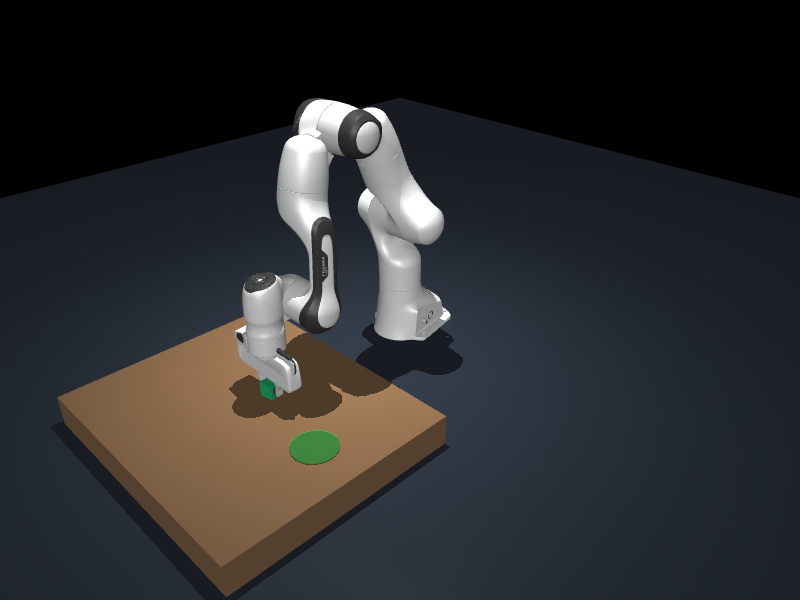
\includegraphics[width=.34\linewidth,height=42mm,keepaspectratio]{figures/soft_grasp.png}\hfill
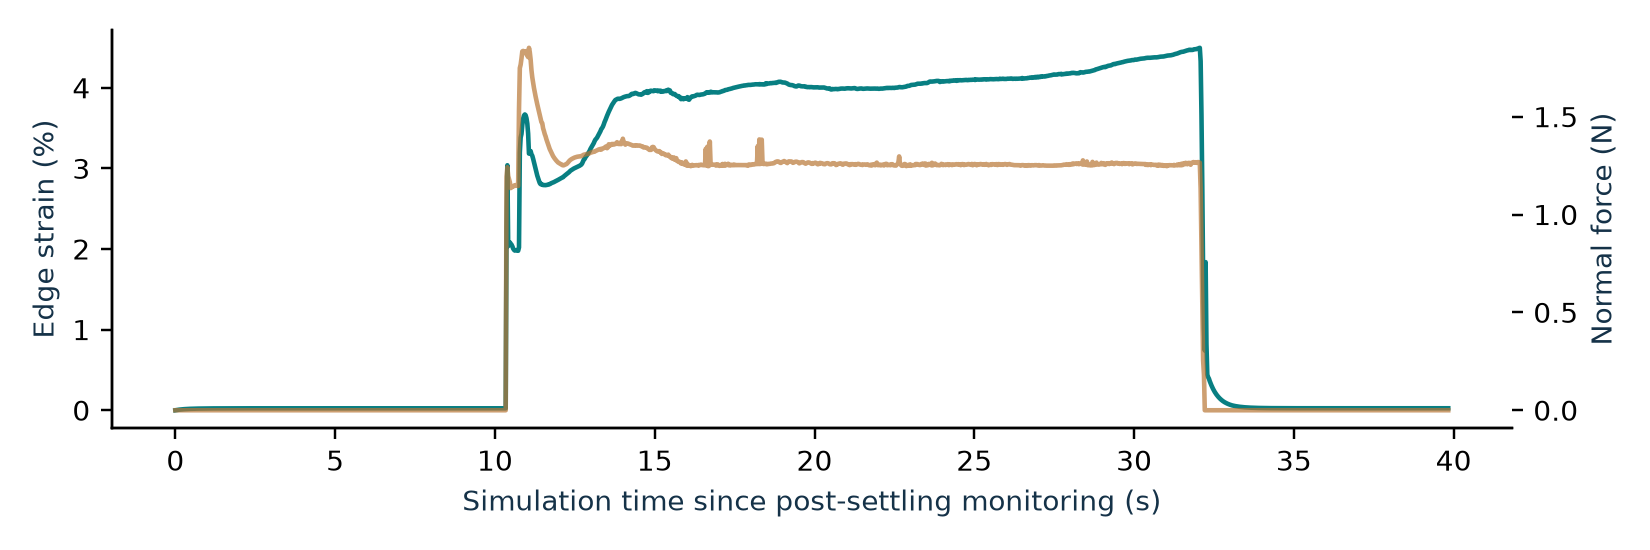
\includegraphics[width=.62\linewidth,height=50mm,keepaspectratio]{figures/soft_trace.png}
\captionof{figure}{Elastic contact and an actual force/strain trace from the root-43 development run. This trace illustrates the mechanism; it is not the mean of the six formal trials.}
\end{center}

\begin{tabularx}{\linewidth}{@{}Yccc@{}}
\toprule Paired experiment & Fixed & Adaptive & Main observed change \\
\midrule Elastic transfer & 2/6 & 6/6 & Four contact-loss failures recovered \\
Rigid uncertain load & 10/12 & 12/12 & Two contact-loss failures recovered \\
\bottomrule
\end{tabularx}

For soft objects, mean episode-maximum absolute edge strain rises from 3.67\% to 4.90\%. The adaptive method completes more transfers within the 40\% gate; it does \emph{not} demonstrate lower deformation. Failed fixed episodes also have shorter exposure. For rigid objects, actual mass varies over 80--250 g, friction over 0.30--0.85 and actuator delay over 0--6 physics steps (0--12 ms at 2 ms/step). These parameters are applied to the physical model and paired exactly. Mean episode-maximum finger normal force increases from 3.16 N to 5.03 N. Force regulation is therefore interpreted as a retention intervention with a contact-load tradeoff.
\takeaway{Completion improves in these sampled material ranges, but retention and gentleness are separate objectives. A future controller should explicitly optimize both slip risk and deformation.}

\newpage
\pageheading{5}{RQ2: why more depth samples can be worse}
\subhead{Observation model and template-free geometry}
Procedural sensing tests use three fixed virtual views of an $80\!\times\!80$ calibrated orthographic ray grid. The observer receives unmasked scene points, removes points near the known support plane, and selects a voxel-connected component near a predeclared workspace hint $(0.48,-0.035)$ m. An 181-angle minimum-area footprint search estimates yaw and horizontal extent; percentile bounds reduce sensitivity to extremes. The underside is approximated by the table. No target class, CAD model or instance label enters grasp estimation, but known calibration, support plane and workspace remain priors. Simulator geometry is still used for planning and transfer.

\begin{tabularx}{\linewidth}{@{}p{43mm}Y@{}}
\toprule Error component & Frozen adverse condition \\
\midrule Missing returns & 35\% independent dropout; persistent periodic missing stripes occupy 22\% of a period. \\
Noise and drift & 1 mm independent Gaussian noise; additional AR(1) drift coefficient 0.85. \\
Outliers and calibration & 4\% z outliers within $\pm25$ mm; fixed per-axis translation bias within $\pm2$ mm. \\
Packet budget & Single packet versus 24 packets: eight per view from three views. Raw and robust fusion use the same packet stream. \\
\bottomrule
\end{tabularx}

\subhead{Cross-packet support instead of indiscriminate accumulation}
Raw fusion concatenates all 24 packets. Robust fusion quantizes points into 4 mm voxels and keeps a voxel only if at least three \emph{different packets} support it, then uses its median point. Multiple points in one packet cannot satisfy the temporal-support threshold. This suppresses transient outliers; it does not guarantee statistically independent packets or remove persistent bias. The paired comparisons verify initial state, object/material seeds and the first corrupted packet SHA-256.

\begin{center}
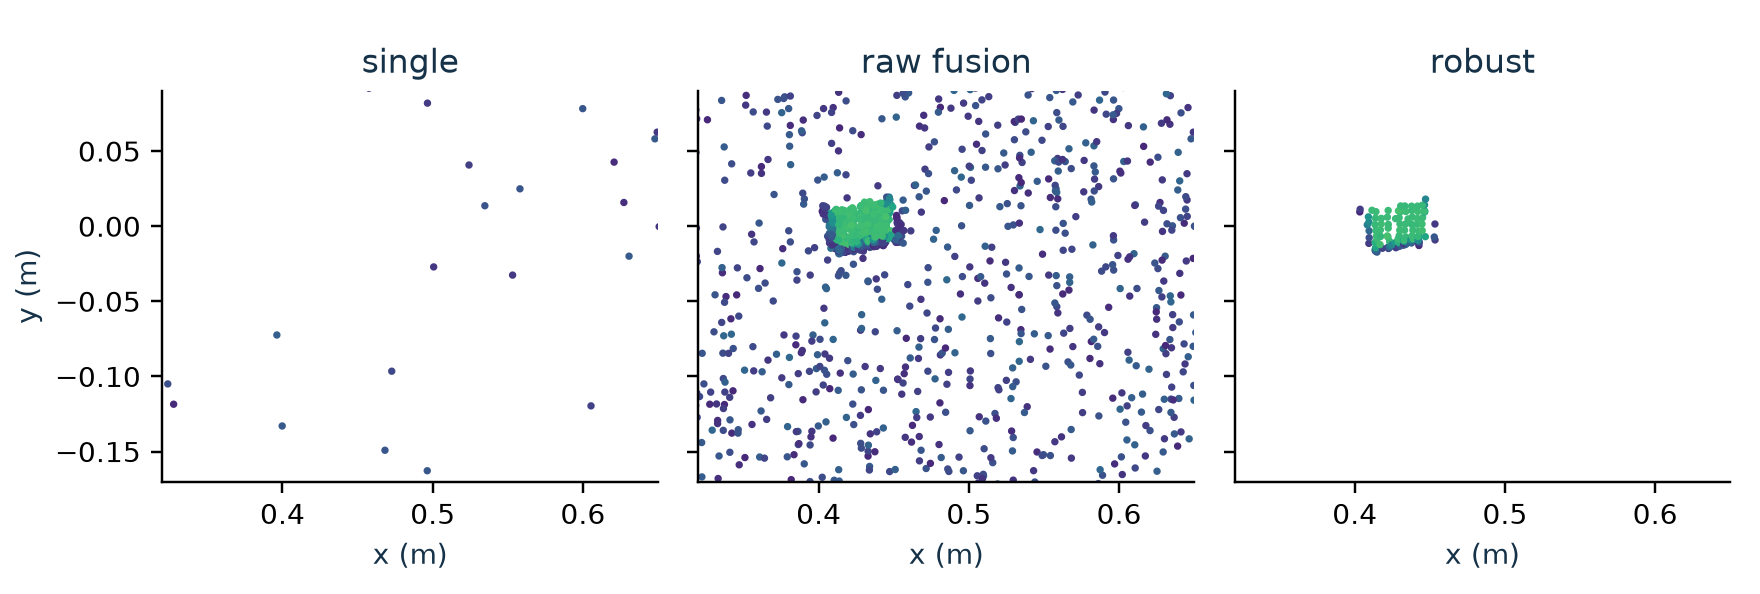
\includegraphics[width=.97\linewidth,height=53mm,keepaspectratio]{figures/corrupted_points.png}
\captionof{figure}{Actual development observations: raw concatenation can join outlier foreground into oversized clusters; cross-packet support suppresses many transient points. Displayed data use no target instance labels.}
\end{center}

\begin{tabularx}{\linewidth}{@{}Yccc@{}}
\toprule Method & Success & 95\% Wilson interval & Recorded failures \\
\midrule Single packet & 6/12 & 25.4--74.6\% & 6 perception \\
Raw 24-packet fusion & 1/12 & 1.5--35.4\% & 11 planning \\
Robust 24-packet fusion & 9/12 & 46.8--91.1\% & 3 contact-loss \\
\bottomrule
\end{tabularx}
Accumulated outliers can connect false foreground into an implausible component, consistent with the raw method's planning failures. All robust failures are wedges (trials 1, 5, 9); its other nine instances succeed. This suggests the limiting stage shifts from usable geometry to contact stability, but the experiment does not separately identify the causal effects of shape and residual estimation error. Synthetic ray corruption and alpha transparency do not model glass refraction or a calibrated physical depth sensor.
\takeaway{The relevant resource is consistent geometric support, not frame count alone. The strongest observation here is the failure of naive fusion, followed by a bounded consistency filter.}

\newpage
\pageheading{6}{RQ3: detecting a real fault and retrying safely}
\subhead{A transient fault that is physically executed}
The first closure in this controlled test is commanded to stop at a 58 mm aperture, wider than the 40 mm target. The robot still executes its planned approach and partial closure. Absent bilateral contacts cause \code{GRASP_FAIL}; no success flag or contact record is fabricated. The fault is transient and is not injected on the second closure. The one-attempt and two-attempt arms share the same fault, initial state and physics. This isolates recovery under a declared command fault rather than estimating a natural failure distribution.

\subhead{Bounded recovery with one evolving scene}
After a permitted failure, the controller opens the jaws, collision-checks a 120 mm upward withdrawal, checks the return-home motion, reobserves and attempts another grasp. Unsafe withdrawal aborts. The scene is initialized exactly once; object state is not restored between attempts. Recovery is permitted only for the declared perception, preflight-planning and grasp-failure stages, not arbitrary slip, collision or transfer failures. Candidate rejections during preflight are distinct from executed grasp attempts.

\begin{center}
\fbox{\parbox{.90\linewidth}{\small
\textbf{Episode record}\quad Initialize once $\rightarrow$ observe/plan $\rightarrow$ partial closure $\rightarrow$ detect missing contacts $\rightarrow$ open and checked retreat $\rightarrow$ reobserve $\rightarrow$ physical regrasp $\rightarrow$ lift/hold $\rightarrow$ release and verify.\\[4pt]
\textbf{Limits}\quad At most two attempts in this study; no robot--object weld; no scene reset between them.}}
\end{center}

\begin{tabularx}{\linewidth}{@{}Yccc@{}}
\toprule Fault experiment & First attempt & Final episode & 95\% Wilson interval \\
\midrule One attempt & 0/6 & 0/6 & 0.0--39.0\% \\
Checked retry & 0/6 & 6/6 & 61.0--100.0\% \\
\bottomrule
\end{tabularx}

\begin{center}
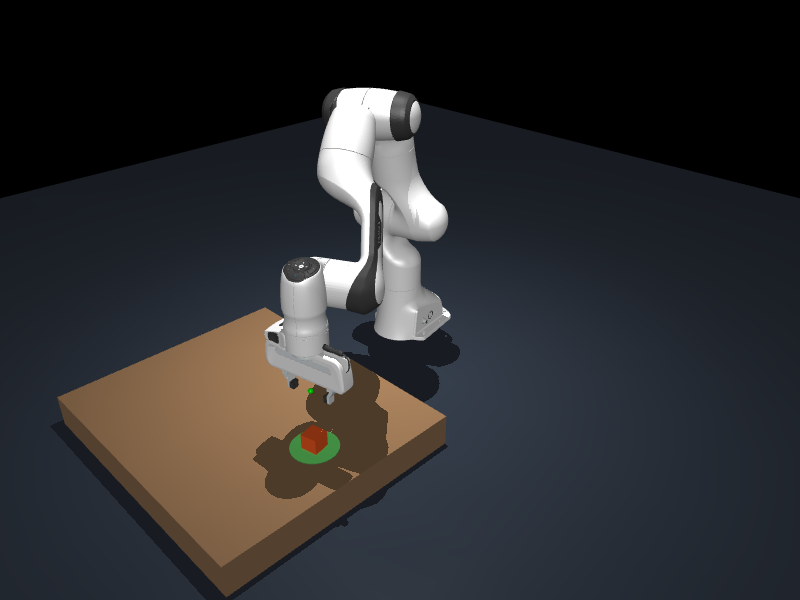
\includegraphics[width=.65\linewidth,height=58mm,keepaspectratio]{figures/recovery_place.png}
\captionof{figure}{Physical release after a failed first closure and a successful second grasp in the root-43 development recording. The video plan preserves the continuous failure--withdrawal--retry sequence.}
\end{center}

\subhead{Interpreting the result correctly}
All six first attempts fail as designed and all six retry episodes complete the task on attempt two. This verifies fault detection, safe state progression and recovery from a temporary closure error. It does not establish a 100\% recovery rate for naturally occurring grasp failures. An unreachable pose remains unreachable, and a dropped object or unsafe retreat can require a different recovery action. The mechanism would need additional fault families, persistent faults and explicit safety-abort controls before broader reliability claims are justified.

\takeaway{A recovery demonstration must show the failed physical action and the subsequent state-preserving retry. Merely rerunning a freshly reset successful scene would answer a different question.}

\newpage
\pageheading{7}{Breadth of exploration and complete screening results}
\subhead{Additional directions, with explicit scope}
\textbf{Stronger clutter/occlusion.} Five live YCB neighbors, reduced spacing, barrier/posts and a physical side screen create at least one view with less than 50\% target visibility per scene. One other view remains fully visible in these trials; this is not all-view occlusion. Single-view success is 5/6 versus active 3/6. Both reject trial 1; active trials 2 and 3 finish 339 mm and 68 mm from the destination. Higher geometric confidence therefore does not ensure complete task success, and the data do not isolate perception as the sole cause of those placement failures.

\textbf{Passive articulation.} A 60 g base and 15 g lid are joined by a dynamic hinge, with range $[-1.2,0]$ rad and randomized initial angle $[-0.8,-0.3]$ rad. All 6/6 whole-assembly tasks succeed; mean hinge excursion is 0.124 rad ($7.1^\circ$). This demonstrates carrying a freely articulated object, not deliberate opening or closing.

\textbf{Procedural unknown shapes.} Tapered, asymmetric, notched and wedge families use seeded random dimensions. Wedges were held out from early tuning; there is no learned training set. Both a generic 40 mm box-prior grasp model and measured point geometry complete 11/12, with the same trial-5 slip. CAD-free estimation is implemented, but its success-rate advantage is not established on this restricted instance set.

\subhead{All 14 conditions: separate 126-episode study}
\begin{center}
{\small
\begin{tabularx}{\linewidth}{@{}p{45mm}cp{25mm}Y@{}}
\toprule Condition & Complete & 95\% Wilson (\%) & Failure counts \\
\midrule
Crowding / single & 5/6 & 43.6--97.0 & planning fail: 1 \\
Crowding / active & 3/6 & 18.8--81.2 & planning fail: 1, place fail: 2 \\
Passive hinge & 6/6 & 61.0--100.0 & None \\
Soft / fixed preload & 2/6 & 9.7--70.0 & slip detected: 4 \\
Soft / force regulation & 6/6 & 61.0--100.0 & None \\
Novel / box prior & 11/12 & 64.6--98.5 & slip detected: 1 \\
Novel / measured points & 11/12 & 64.6--98.5 & slip detected: 1 \\
Rigid / fixed preload & 10/12 & 55.2--95.3 & slip detected: 2 \\
Rigid / force regulation & 12/12 & 75.7--100.0 & None \\
Fault / one attempt & 0/6 & 0.0--39.0 & grasp fail: 6 \\
Fault / checked retry & 6/6 & 61.0--100.0 & None \\
Depth / single packet & 6/12 & 25.4--74.6 & perception fail: 6 \\
Depth / raw fusion & 1/12 & 1.5--35.4 & planning fail: 11 \\
Depth / robust fusion & 9/12 & 46.8--91.1 & slip detected: 3 \\
\bottomrule
\end{tabularx}

}
\end{center}
The formal exploratory root seed is 20261026, distinct from development seeds 1, 2, 3, 43 and 1044. Conditions are paired on the same initial generalized coordinates or full settled scene, actual material parameters and object-instance seed. Sensor comparisons additionally retain packet hashes. Every outcome remains in the denominator. The 126 exploratory episodes and 180 candidate-ablation episodes address different questions and are not pooled into one success rate.
\takeaway{Coverage is not equivalent to a solved research field. The negative active-view result, tied unknown-shape result and residual wedge slips identify concrete next experiments.}

\newpage
\pageheading{8}{Evidence strength, failures and next experiments}
\subhead{Small samples and paired comparisons}
For $k$ successes from $n$ episodes, the report uses a Wilson binomial interval with $z=1.96$:
\begin{equation}
\frac{\widehat p+z^2/(2n)\ \pm\ z\sqrt{\widehat p(1-\widehat p)/n+z^2/(4n^2)}}{1+z^2/n},\qquad \widehat p=k/n.
\end{equation}
Even 6/6 corresponds to a 61.0\% lower endpoint, and 12/12 to 75.7\%; neither proves universal reliability. Exact paired McNemar tests use discordant scenes, not an unpaired comparison of percentages. For the seven predeclared exploratory comparisons, raw $p$ values are 0.5 (crowding), 0.125 (soft), 1.0 (novel), 0.5 (force), 0.03125 (recovery), 0.125 (single/raw), and 0.0078125 (raw/robust). Bonferroni's threshold is $0.05/7\approx0.00714$, so none passes; the smallest adjusted $p$ is 0.0546875. The 180-episode candidate study is analyzed separately, with $p=0.125$ and 0.25. We report observed differences and mechanism evidence, not statistically established population improvements.

\subhead{Failure localization and falsifiable follow-up}
\begin{tabularx}{\linewidth}{@{}p{28mm}Y Y@{}}
\toprule Finding & Evidence-supported interpretation & Next controlled experiment \\
\midrule Blocked approach & Original palm geometry collides; bounded alternatives recover specific scenes. & Sweep clearance/offset under fixed scenes, holding candidate budget constant. \\
Raw fusion collapse & 11/12 planning failures; accumulated false support can distort the foreground cluster. & Factor outliers, stripes and drift separately; compare equal packet budgets. \\
Robust wedge slips & All three residual robust failures are wedges. & Factor geometry error and friction with oracle/measured-observation arms. \\
Soft retention/strain & More complete tasks, higher mean peak strain. & Equal-duration exposure; sweep force target and deformation-aware stopping. \\
Active-view regression & Two additional placement failures despite accepted estimates. & Replay paired trajectories and estimate errors before assigning causation. \\
Transient fault recovery & Six controlled failures recovered without scene reset. & Add persistent closure faults and withdrawal obstacles; require safe abort. \\
\bottomrule
\end{tabularx}

\subhead{External validity and measurement boundaries}
The workcell is synthetic and structured. Known calibration, upright/template priors in clutter, a workspace hint in point-only sensing, simulator collision maps and true transfer centering simplify the task. Transparency is an appearance/corruption setting, not glass optics. The elastic model is uncalibrated, and the articulated policy does not manipulate the joint deliberately. Contact-force readings are simulator values. Discrete motion checks do not prove real-robot safety; there is no hardware transfer or real camera timing experiment. Neighbor translation is bounded after settling, but independent rotation or surface damage limits are not defined. Timing from overlapping experimental processes is not used for hardware efficiency comparisons.

\takeaway{The defensible contribution is a set of localized questions, bounded algorithms, preserved failures and reproducible physical checks. These provide stronger evidence than a montage of selected successes.}

\newpage
\pageheading{9}{Reproduction, verification and references}
\subhead{Run the principal functions}
Use Python 3.12. Core requirements pin MuJoCo 3.15.0 and NumPy 2.5.3. Frozen experiments record Python 3.12.15; the present verification uses Python 3.12.4. Bundled model assets include licenses and lock files; neither Python nor installed dependency wheels are included. From the project root:
{\small
\begin{verbatim}
py -3.12 -m venv .venv
.venv\Scripts\python -m pip install -r requirements.txt
.venv\Scripts\python scripts/setup_assets.py
.venv\Scripts\python scripts/setup_ycb.py
.venv\Scripts\python demo_viewer.py
.venv\Scripts\python main.py --headless --balanced --task place --trials 6
.venv\Scripts\python clutter_main.py --headless --scene dense --trials 3
.venv\Scripts\python exploration_main.py --case sensor_robust --trials 3
.venv\Scripts\python exploration_main.py --case soft_adaptive --trials 3
.venv\Scripts\python exploration_main.py --case recovery_retry --trials 3
\end{verbatim}}
The GUI selects a case and starts a fresh run; pre-recorded footage is separate. For the fixed protocol, use \code{scripts/benchmark_completion.py --output outputs/new_completion --workers 1} and \code{scripts/benchmark_exploration.py --output outputs/new_exploration}; use new directories and retain all failures. Rendering is optional. The bundled video plan gives exact source clips, speed labels and a 300-second narration schedule; development clips are excluded from experimental denominators.

\subhead{Verified evidence and deliverable map}
All 49 automated tests pass, including physical release, genuine flex deformation, a freely moving hinge, observer input isolation, checked retry and rejection of forged/stale evidence. Both current evidence audits pass: 180 paired candidate episodes and 126 exploratory episodes. These are audits of existing frozen records plus functional tests; they are not 306 newly sampled trials. Complete protocol/JSONL/comparison files are in \code{docs/validation/v2.1.0} and \code{docs/validation/v3.0.0}. The engine is unchanged for this report revision.

{\scriptsize
\begin{tabularx}{\linewidth}{@{}p{25mm}Y@{}}
\toprule Evidence & Frozen source SHA-256 \\
\midrule Candidate study & \code{0f386f1f87282a2e9485fc9254487ca93a4f58c04f614627816926a1300005b9} \\
Exploratory study & \code{9f59c29b6dc0a62c15d10249788590491010c02d32f9ed1baf884d871e08c418} \\
\bottomrule
\end{tabularx}}

LaTeX source and local figures are in \code{docs/final_report}; the compiled report is \code{output/pdf/EE5110_Final_Report.pdf}. Build with \code{scripts/build_final_report.py --engine tectonic}, or upload the source folder to Overleaf. Video narration, subtitles and the Chinese editing guide are in \code{docs/final_video}. Code/requirements/assets and both frozen studies accompany the review package; SHA-256 and archive CRC checks detect incomplete transfers. Group identities and individual contribution statements must be supplied from actual team records.

\vspace{-3pt}
\begin{thebibliography}{6}\small\setlength{\itemsep}{1pt}\setlength{\parskip}{0pt}
\bibitem{brief} EE5110 Segment C, \emph{CA: Robotic Grasping Simulation}, course brief supplied by the instructor, 2026. Required: report, introduction/demo video, source and run instructions in one ZIP.
\bibitem{mujoco} MuJoCo documentation, \emph{XML Reference: flexcomp and elasticity}. \url{https://mujoco.readthedocs.io/en/stable/XMLreference.html}. Accessed 27 Oct. 2026.
\bibitem{menagerie} Google DeepMind, \emph{MuJoCo Menagerie: Franka Emika Panda}. \url{https://github.com/google-deepmind/mujoco_menagerie}. Asset commit pinned in \code{assets/panda.lock.json}.
\bibitem{ycb} B. Calli et al., ``Benchmarking in Manipulation Research: The YCB Object and Model Set and Benchmarking Protocols,'' 2015. \url{https://arxiv.org/abs/1502.03143}.
\bibitem{conversion} elpis-lab, \emph{YCB\_Dataset}, simulation asset conversion, commit \code{9e8c6488a2ff673d9aa48a91492fb89423c1b106}. \url{https://github.com/elpis-lab/YCB_Dataset}. Original notices retained.
\bibitem{project} Project source, protocols and frozen records. \url{https://github.com/m13961023616-pixel/EE5110-SegC}. Base revision \code{f65ee0c}; analysis/report revision on a separate branch.
\end{thebibliography}
\end{document}
